\newpage
\section{Durchführung}
\label{sec:durchfuehrung}

\subsection{Aufbau}
In diesem Versuch wird das Sagnac-Interferometer verwendet, dessen schematischer Aufbau in \autoref{fig:schema} dargestellt ist.

\begin{figure}[H]
    \centering
    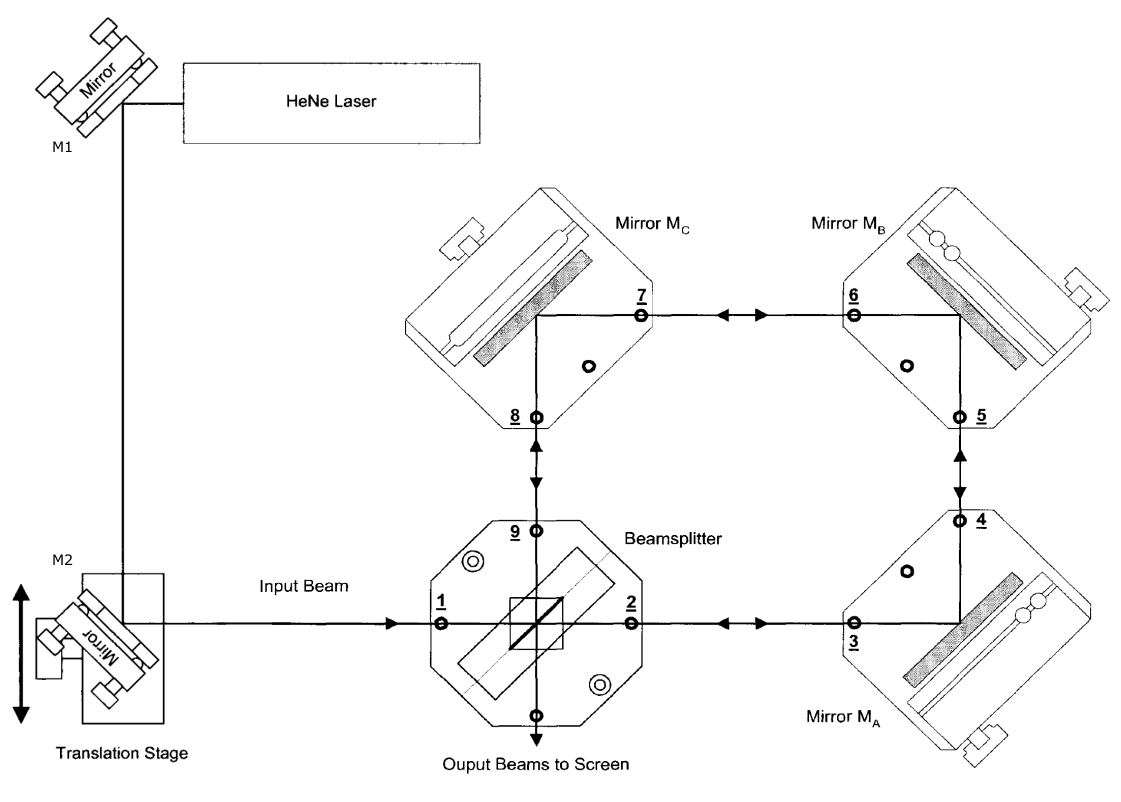
\includegraphics[scale=0.37]{images/aufbau_schema.png}
    \caption{Schematische Darstellung des Sagnac-Interferometers.\cite{V64}}
    \label{fig:schema}
\end{figure}

Am Strahlausgang des Interferometers sitzt ein weiterer Strahlteilerwürfel, dessen zwei linear polarisierte Strahlen in zwei separate Photodioden-Detektoren führen.
Da der schematische Aufbau nur das Sagnac-Interferometer zeigt, müssen für den Versuch zusätzliche optische Elemente eingebaut werden.
Je nach Durchführungsabschnitt werden ein Polarisationsfilter, Glasplättchen oder eine Gaszelle zusätzlich im Strahlengang verbaut.
Ein Polarisationsfilter wird vor das Interferometer in \SI{45}{\degree}-Stellung in den Strahl gestellt, um nur diese Komponente des linear polarisierten Laserlichts durchzulassen.
Das genutzte Laserlicht wird in einem He-Ne Laser erzeugt und besitzt die Wellenlänge \SI{632.990}{\nano\metre}.
Hinter dem Polarisationsfilter führt der Strahl in den Strahlteilerwürfel, der den Strahl in eine linear horizontale und eine linear vertikale Komponente im rechten Winkel aufteilt.
Beide Strahlen haben die gleiche Intensität und propagieren jeweils weiter zu den verstellbaren Spiegeln $M_A$, $M_B$ und $M_C$.
Nach Durchlaufen der selben Wegstrecke beider Strahlen, entweder über $M_A \rightarrow M_B \rightarrow M_C$ oder über $M_C \rightarrow M_B \rightarrow M_A$, treffen Beide wieder auf den Kristall und werden wieder zusammengeführt.\\
Der Aufbau ist, zusätzlich mit einer Lufthaube verkleidet, in \autoref{fig:aufbau} dargestellt.

\begin{figure}[H]
    \centering
    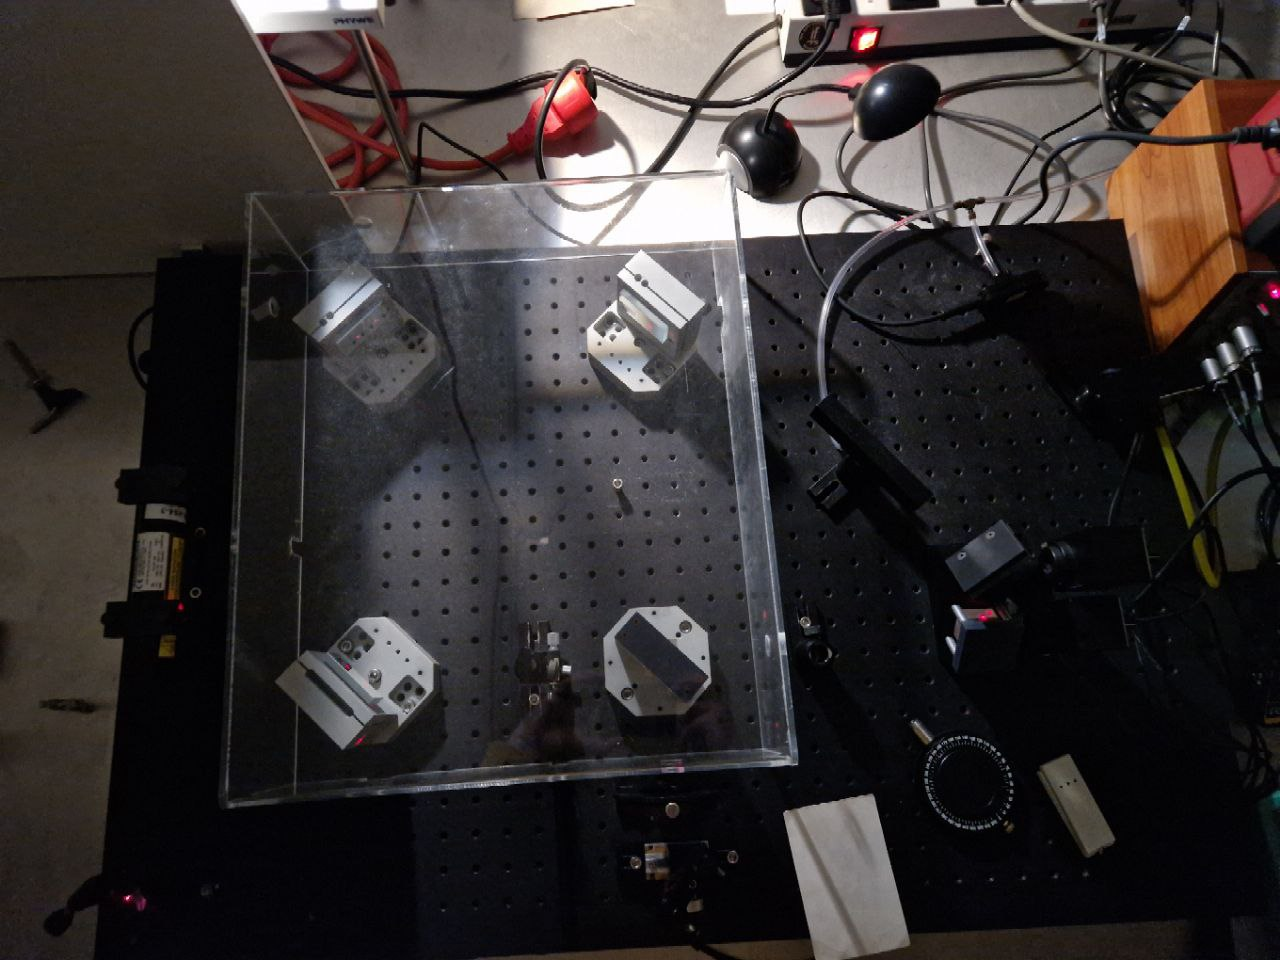
\includegraphics[scale=0.3]{images/aufbau.jpg}
    \caption{Versuchsaufbau des Sagnac-Interferometers nach Justage und dem Einsetzen der Glasplättchen.}
    \label{fig:aufbau}
\end{figure}

\subsection{Justage und Messprogramm}
Um das System zu justieren sind an den drei Spiegel Achsen mit Stellschrauben angebracht.
Es wird jeweils nur einer der zwei Strahlen betrachtet und dessen optischer Pfad justiert.
In alterierender Reihenfolge werden so die Spiegel eingestellt, bis beide Strahlen das Interferometer möglichst parallel verlassen.
Zur Überprüfung der Parallelität wird vor den zweiten Strahlteilerwürfel ein zweiter Polarisationsfilter mit \SI{45}{\degree}-Stellung verbaut und das durchscheinende Licht auf ein Stück Papier projiziert.
Anhand des Interferenzmusters auf dem Papier lässt sich die Parallelität ablesen.
Sind Interferenzstreifen zu erkennen, so treten die Lichtstrahlen unter einem Winkel $\theta \neq \SI{0}{\degree}$ aus dem Interferometer aus.\\
Zur weiteren Justage wird der Spiegel $M_2$, der sich auf einer Schiebeplatte befindet, mit dieser verschoben, sodass die zwei einzelnen linear polarisierten Strahlen im Interferometer räumlich getrennt werden.
Aus diesem Zustand heraus wird erneut justiert, damit auch die räumlich im Interferometer getrennten Strahlen ohne Interferenzstreifen interferieren.
Zwischen Spiegel $M_C$ und dem Strahlteilerwürfel des Interferometers wird nun ein Rotationselement mit zwei Glasscheiben eingesetzt, durch die je einer der Strahlen propagiert.
Der zweite Polarisationsfilter wird entfernt und das Papier ebenfalls, sodass der mit den Photodioden verbundene zweite Strahlteilerwürfel wieder im Interferenzstrahlengang liegt.\\
Die Ausgänge der Photodioden werden an einen sogenannten \textit{Modern Interferometry Controller} angeschlossen, welcher die Differenz beider Signale bildet und es graphisch auf einem Oszilloskop darstellt.
Zusätzlich dazu zählt das MIC wie häufig die Differenz der Signale die \SI{0}{\volt} überschreitet bzw. unterschreitet.
Zuletzt wird die Plastikhaube um das Interferometer samt Glasplättchen gestellt, damit Schwankungen der Luftdichte minimal sind.\\
\newline
Die erste Messung soll den Kontrast der Interferenz nach \autoref{eq:kontrast} in Abhängigkeit des Polarisationswinkels untersuchen.
Dazu wird ein Polarisationswinkel am Polarisationsfilter vor dem Interferometer eingestellt und durch Rotation an den Glasplättchen die Interferenzmaxima und -minima eingestellt.
Dies wird für mehrere Winkel durchgeführt.\\
Für Messung vom Brechungsindex von Glas, wird der Polarisationswinkel auf den Winkel mit maximalem Kontrast eingestellt und fixiert.
In 10 Durchgängen werden nun die Interferenzmaxima und -minima am MIC gezählt, abhängig von der Rotation der Glasplättchen.\\
Als letzte Messung soll der Brechungsindex von Luft bestimmt werden, indem eine Gaszelle anstatt der Glasplättchen in einen Strahlengang im Interferometer verbaut wird.
Der zweite linear polarisierte Strahl soll neben der Gaszelle verlaufen.
Hierzu wird ein Vakuum in der ca $\SI{100.0\pm0.1}{\milli\metre}$ langen Gaszelle angelegt.
Es werden in drei Durchläufen erneut die Anzahl der Interferenzmaxima und -minima am MIC abgelesen, in \SI{50}{\milli\bar} Schritten.
Hierfür soll die Temperatur des Raums notiert werden.